
\chapter{\acl{SKE} Schemes}

\begin{definition}[\acl{SKE} scheme]
	We call $\SKESchemeTuple$ a \ac{SKE} scheme.
	\begin{itemize}
		\item $\SKEKeyGen$ outputs a key $k \rand{\K}$;
		\item $\Enc(k, m) = c$ for some $m \in \M$, $c \in \C$;
		\item $\Dec(k, c) = m$.
	\end{itemize}
	As usual, we want $\SKEScheme$ to be correct.
\end{definition}

We want to introduce computational security: a bounded adversary can not gain information on the message given the cyphertext.
\begin{definition}[One time security]
	A \ac{SKE} scheme $\SKESchemeTuple$ has one time computational security if for all \ac{PPT} adversaries $\Adv$ $\exists$ a negligible function $\epsilon$ such that
	\begin{equation*}
		\abs{
			\Pr{\SKEGameOneTime(\lambda, 0) = 1}
			-
			\Pr{\SKEGameOneTime(\lambda, 1) = 1}
		}
		\le \epsilon(\lambda)
	\end{equation*}
	where $\SKEGameOneTime(\lambda, b)$ is the following ``game'' (or experiment):
	\begin{enumerate}
		\item pick $k \rand{\K}$;
		\item $\Adv$ outputs two messages $(m_0, m_1) \from \Adv(1^{\lambda})$ where $m_0, m_1 \in \M$ and $\abs{m_0} = \abs{m_1}$;
		\item $\c = \SKEEnc(k, m_b)$ with $b$ input of the experiment;
		\item output $b' \from \Adv(1^{\lambda}, c)$, \ie the adversary tries to guess which message was encrypted. \qedhere
	\end{enumerate}
\end{definition}

Let's look at a construction.
\begin{construction}[\acs{SKE} scheme from \acs{PRG}] \label{cons:ske-prg}
	Let $\G : \{0,1\}^{n} \to \{0,1\}^{l}$ be a \ac{PRG}.
	Set $\K = \{0,1\}^{n}$, and $\M = \C = \{0,1\}^{l}$.
	Define $\SKEEnc(k,m) = \G(k) \xor m$ and $\SKEDec(k,c) = \G(k) \xor c$.
\end{construction}

\begin{theorem} \label{thm:ske-prg}
	If $\G$ is a \ac{PRG}, the \ac{SKE} in \cref{cons:ske-prg} is one-time computationally secure.
\end{theorem}

\begin{proof}[Proof of \cref{thm:ske-prg}]
	Consider the following experiments:
	\begin{itemize}
		\item $\H_0(\lambda, b)$ is like $\SKEGameOneTime$:
		\begin{enumerate}
			\item $k \rand{\{0,1\}^{n}}$;
			\item $(m_0, m_1) \from \Adv(1^{\lambda})$;
			\item $c = \G(k) \xor m_b$;
			\item $b' \from \Adv(1^{\lambda}, c)$.
		\end{enumerate}
		\item $\H_1(\lambda, b)$ replaces $\G$ with something truly random:
		\begin{enumerate}
			\item $(m_0, m_1) \from \Adv(1^{\lambda})$;
			\item $r \rand{\{0,1\}^{l}}$;
			\item $c = r \xor m_b$, basically like \ac{OTP};
			\item $b' \from \Adv(1^{\lambda}, c)$.
		\end{enumerate}
		\item $\H_2(\lambda)$ is just randomness:
		\begin{enumerate}
			\item $(m_0, m_1) \from \Adv(1^{\lambda})$;
			\item $c \rand{\{0,1\}^{l}}$;
			\item $b' \from \Adv(1^{\lambda}, c)$.
		\end{enumerate}
	\end{itemize}

	First, we show that $\H_0(\lambda, b) \CompInd \H_1(\lambda, b)$, for $b \in \{0,1\}$.
	Fix some value for $b$, and assume exists a \ac{PPT} distinguisher $\Distinguisher$ between $\H_0(\lambda, b)$ and $\H_1(\lambda, b)$: we then can construct a distinguisher $\Distinguisher'$ for the \ac{PRG}.

	$\Distinguisher'$, on input $z$, which can be either $\G(k)$ for some $k \rand{\{0,1\}^{n}}$, or directly $z \rand{\{0,1\}^{l}}$, does the following:
	\begin{itemize}
		\item get $(m_0, m_1) \from \Distinguisher(1^{\lambda})$;
		\item feed $z \xor m_b$ to $\Distinguisher$;
		\item output the result of $\Distinguisher$.
	\end{itemize}

	Now, we show that $\H_1(\lambda, b) \CompInd \H_2(\lambda, b)$, for $b \in \{0,1\}$.
	By perfect secrecy of \ac{OTP} we have that $(m_0 \xor r) \approx z \approx (m_1 \xor r)$, so $\H_1(\lambda, 0) \CompInd H_2(\lambda) \CompInd \H_1(\lambda, 1)$.
\end{proof}

\begin{corollary}
	One-time computationally secure \ac{SKE} schemes are in Minicrypt.
\end{corollary}

This scheme is not secure if the adversary knows a $(m_1, c_1)$ pair, and we reuse the key.
Take any $m, c$, then $c \xor c_1 = m \xor m_1$, and you can find $m$.
This is called a \ac{CPA}, something we will defined shortly using a \ac{PRF}.

\section{\aclp{CPA} and \aclp{PRF}}

\begin{definition}[\acl{PRF}]
	Let $\F = \{ F_k : \{0,1\}^{n} \to \{0,1\}^{l} \}$ be a family of functions, for $k \in \{0,1\}^{\lambda}$.
	Consider the following two experiments:
	\begin{itemize}
		\item $\PRFGameReal(\lambda)$, defined as:
			\begin{enumerate}
				\item $k \rand{\{0,1\}^{\lambda}}$;
				\item $b' \from \Adv^{F_k(\cdot)}(1^{\lambda})$, where $\Adv$ can query an oracle for values of $F_k(\cdot)$, without knowing $k$.
			\end{enumerate}
		\item $\PRFGameRand(\lambda)$, defined as:
			\begin{enumerate}
				\item $R \rand{\R(n \to l)}$, \ie a function $R$ is chosen at random from all functions from $\{0,1\}^{n}$ to $\{0,1\}^{l}$;
				\item $b' \from \Adv^{R(\cdot)}(1^{\lambda})$, where $\Adv$ can query an oracle for values of $R(\cdot)$.
			\end{enumerate}
	\end{itemize}
	The family $\F$ of functions is a \ac{PRF} family if for all \ac{PPT} adversaries $\Adv$ $\exists$ a negligible function $\epsilon$ such that
	\begin{equation*}
		\abs{
			\Pr{\PRFGameReal(\lambda) = 1}
			-
			\Pr{\PRFGameRand(\lambda) = 1}
		}
		\le \epsilon(\lambda). \qedhere
	\end{equation*}
\end{definition}

To introduce \acp{CPA} and \ac{CPA}-secure \ac{SKE} schemes, we first introduce the game of \ac{CPA}.
As usual, a \ac{SKE} scheme is a tuple $\SKESchemeTuple$.

\begin{definition}[\acs{CPA}-secure \acs{SKE} scheme]
	Let $\SKESchemeTuple$ be a \ac{SKE} scheme, and consider the game $\CPAGame(\lambda, b)$, defined as:
	\begin{enumerate}
		\item $k \rand{\{0,1\}^{\lambda}}$;
		\item $(m_0, m_1) \from \Adv^{\SKEEnc(k, \cdot)} (1^{\lambda})$.
			$\Adv$ is given access to an oracle for $\SKEEnc(k, \cdot)$, so she knows some $(m,c)$ couples, with $c = \SKEEnc(k, m)$;
		\item $c \from \SKEEnc(k, m_b)$;
		\item $b' \from \Adv^{\SKEEnc(k, \cdot)}(1^{\lambda}, c)$.
	\end{enumerate}

	$\SKEScheme$ is \ac{CPA}-secure if for all \ac{PPT} adversaries $\Adv$
	\begin{equation*}
		\CPAGame(\lambda, 0) \CompInd \CPAGame(\lambda, 1). \qedhere
	\end{equation*}
\end{definition}

Deterministic schemes cannot achieve this, \ie when $\SKEEnc$ is deterministic the adversary could cipher $m_0$ and then compare $c$ to $\SKEEnc(k, m_0)$, and output $0$ if and only if $c = \SKEEnc(k, m_0)$.

Let's construct a \ac{CPA}-secure \ac{SKE} scheme using \acp{PRF}.
\begin{construction}[\acs{SKE} scheme from \acs{PRF}] \label{cons:ske-prf}
	Let $\F$ be a \ac{PRF}, we define the following \ac{SKE} scheme $\SKESchemeTuple$:
	\begin{itemize}
		\item $\SKEKeyGen$ takes $k \rand{\{0,1\}^{\lambda}}$;
		\item $\SKEEnc(k,m) = (r, F_k(r) \xor m)$, with $r \rand{\{0,1\}^{n}}$.
			Note that, since $F_k : \{0,1\}^{n} \to \{0,1\}^{l}$, we have that $\M = \{0,1\}^{l}$ and $\C = \{0,1\}^{n+l}$;
		\item $\SKEDec(k, (c_1, c_2)) = F_k(c_1) \xor c_2$. \qedhere
	\end{itemize}
\end{construction}

Our construction is both one time computationally secure, and secure against \acp{CPA}.
\begin{theorem} \label{thm:ske-prf-cpa}
	If $\F$ is a \ac{PRF}, \cref{cons:ske-prf} is \ac{CPA}-secure.
\end{theorem}

\begin{proof}[Proof of \cref{thm:ske-prf-cpa}]
	First, we define the experiment $\H_0(\lambda, b) \equiv \CPAGame(\lambda, b)$ as follows:
	\begin{enumerate}
		\item $k \rand{\{0,1\}^{\lambda}}$;
		\item $(m_0,m_1) \from \Adv^{\SKEEnc(k, \cdot)} (1^{\lambda})$;
		\item $c^{\star} \from (r^{\star}, F_k(r^{\star}) \xor m_b)$, where $r^{\star} \rand{\{0,1\}^{n}}$;
		\item output $b' \from \Adv^{\SKEEnc(k, \cdot)} (1^{\lambda}, c^{\star})$.
	\end{enumerate}
	Note that in the \ac{CPA} game the adversary has access to an encryption oracle using the chosen key.

	Now, for the first hybrid $\H_1(\lambda, b)$, where we sample a random function $R$ in place of $F_k$:
	\begin{enumerate}
		\item $R \rand{\R(n \to l)}$;
		\item $(m_0,m_1) \from \Adv^{\SKEEnc(R, \cdot)} (1^{\lambda})$, where now $\SKEEnc(R, m) = (r, R(r) \xor m)$ for some random $r$;
		\item $c^{\star} \from (r^{\star}, R(r^{\star}) \xor m_b)$, where $r^{\star} \rand{\{0,1\}^{n}}$;
		\item output $b' \from \Adv^{\SKEEnc(R, \cdot)} (1^{\lambda}, c^{\star})$.
	\end{enumerate}

	Our first claim is that $\H_0(\lambda, b) \CompInd \H_1(\lambda, b)$ for $b \in \{0,1\}$.
	As usual, we assume that exists an adversary $\Adv$ which can distinguish the experiments, \ie that can distinguish the oracles, and use $\Adv$ to create $\Adv_{\text{PRF}}$ that breaks the \ac{PRF}.

	$\Adv_{\text{PRF}}$ has access to some oracle $O(\cdot)$, with is one of two possibilities:
	\begin{equation*}
		O(x) =
		\begin{cases}
			F_k(x) & \text{ for } k \rand{\{0,1\}^{\lambda}} \\
			R(x) & \text{ for } R \rand{\R(n \to l)}.
		\end{cases}
	\end{equation*}
	$\Adv$ gives $\Adv_{\text{PRF}}$ some message $m$.
	$\Adv_{\text{PRF}}$ picks $r \rand{\{0,1\}^{n}}$, and queries $O(r)$ to get $z \in \{0,1\}^{l}$.
	Then it gives $(r, z \xor m)$ to $\Adv$.
	This is repeated as long as $\Adv$ asks for encryption queries.

	Then $\Adv$ gives to $\Adv_{\text{PRF}}$ $(m_0, m_1)$, which repeats the same procedure using $m_0$ as a message (to distinguish $\H_0(\lambda, 0)$ from $\H_1(\lambda, 0)$) to compute $c^{\star}$.
	$\Adv$, after receiving $c^{\star}$, asks some more encryption queries, and then outputs $b'$.
	If $b' = 1$, $\Adv_{\text{PRF}}$ says $R(\cdot)$, otherwise it says $F_k(\cdot)$.

	Now for the third experiment, $\H_2(\lambda)$, which uses $\PKEEnc(m) = (r_1, r_2)$ with $(r_1, r_2) \rand{\{0,1\}^{n+l}}$, \ie it outputs just randomness.

	Our second claim is that $\H_1(\lambda, b) \CompInd \H_2(\lambda)$ for $b \in \{0,1\}$.
	To see this, note that $\H_1$ and $\H_2$ are identical as long as collisions don't happen when choosing the $r$s.
	It suffices for us to show that collisions happen with small probability.

	Call $E_{i,j}$ the event ``random $r_i$ collides with random $r_j$''.
	The event of a collision is thus $E = \biglor_{i,j} E_{i,j}$, and its probability can be upper bounded as follows:
	\begin{equation*}
		\Pr{E} = \sum_{i,j} \Pr{E_{i,j}} = \sum_{i,j} \Coll\left(\U_n\right) \le \binom{q}{2} 2^{-n} \le \frac{q^{2}}{2^{n}}
	\end{equation*}
	where $q$ is the (polynomial) number of queries that the adversary does, and $\Coll\left(\U_n\right)$ is the probability of a collision when using a uniform distribution, which is $2^{-n}$.
\end{proof} 

\begin{theorem}[\acs{GGM}, 1982]
	\acp{PRF} can be constructed from \acp{PRG}.
\end{theorem}

\begin{corollary}
	\acp{PRF} are in Minicrypt.
\end{corollary}

\begin{construction}[\acs{GGM} tree] \label{cons:ggm-tree}
	Assume we have a length doubling \ac{PRG} $\G : \{0,1\}^{\lambda} \to \{0,1\}^{2\lambda}$.
	We say that $\G(x) \Definition (\G_0(x), \G_1(x))$ to distinguish the first $\lambda$ bits from the second $\lambda$ bits.

	\begin{figure}
		\centering
		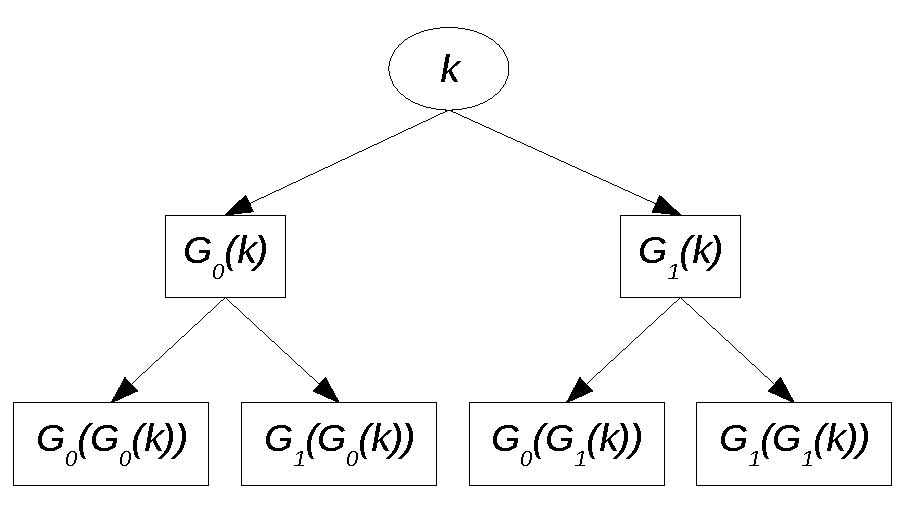
\includegraphics[width=0.8\linewidth]{drawings/ggm-tree.eps}
		\caption{First two levels of a \acs{GGM} tree.}
		\label{fig:ggm-tree}
	\end{figure}

	Now, to build the \ac{PRF} we construct a \ac{GGM} tree (\cref{fig:ggm-tree}) starting with a key $k \in \{0,1\}^{\lambda}$.
	On input $x = (x_1, \dots, x_n) \in \{0,1\}^{n}$, with $n$ being the height of the tree, the \ac{PRF} picks a path in the tree:
	\begin{equation*}
		F_k(x) = \G_{x_n} \left( \dots \G_{x_1}(k) \dots \right).
	\end{equation*}
\end{construction}

\begin{lemma} \label{lem:prg-poly-times}
	Let $\G : \{0,1\}^{\lambda} \to \{0,1\}^{2\lambda}$ be a \ac{PRG}.
	Then for all $t(\lambda) = \poly(\lambda)$ we have that
	\begin{equation*}
		\left( \G(k_1), \dots, \G(k_t) \right)
		\CompInd
		\underbrace{\left( \U_{2\lambda}, \dots, \U_{2\lambda} \right)}_{t \text{ times}}. \qedhere
	\end{equation*}
\end{lemma}

\begin{proof}[Proof of \cref{lem:prg-poly-times}]
	We define $t$ hybrids, where $\H_i(\lambda)$ is defined as
	\begin{equation*}
		\H_i(\lambda) = ( \G(k_1), \dots, \G(k_{t-i}), \underbrace{\U_{2\lambda}, \dots, \U_{2\lambda}}_{i \text{ times}} )
	\end{equation*}
	thus $\H_0(\lambda) = (\G(k_1), \dots, \G(k_t))$ and $\H_t(\lambda) = (\U_{2\lambda}, \dots, \U_{2\lambda})$.
	To prove that $\H_1(\lambda) \CompInd \H_t(\lambda)$, we show that for any $i$ it holds that $\H_i(\lambda) \CompInd \H_{i+1}(\lambda)$.
	This relies on the fact that $\G(k_{t-i}) \CompInd \U_{2\lambda}$: assume that exists a distinguisher $\Distinguisher$ for $\H_{i}(\lambda)$ and $\H_{i+1}(\lambda)$, we then break the \ac{PRG}.

	We build $\Distinguisher'$, which takes in input some $z$ from either $\G(k_{t-i})$ or $\U_{2\lambda}$.
	$\Distinguisher'$ takes $k_1, \dots, k_{t-(i+1)} \rand{\{0,1\}^{\lambda}}$, and feeds $(\G(k_1), \dots, \G(k_{t-(i+1)}), z, \U_{2\lambda}, \dots, \U_{2\lambda})$ to $\Distinguisher$, and returns whatever it returns.
\end{proof}

\begin{proof}[Proof that \cref{cons:ggm-tree} is a \acs{PRF}]
	We'll define a series of hybrids to show that the \ac{GGM} tree is a \ac{PRF}.
	$\H_0(\lambda) \equiv$ our \ac{GGM} tree.

	$\H_i(\lambda)$, for $i \in [1, n]$, will replace the tree up to depth $i$ with a true random function.
	$\H_i(\lambda)$ initially has two empty arrays $T_1$ and $T_2$.
	On input $x \in \{0,1\}^{n}$, it checks if $\vec{x} = (x_1, \dots, x_i) \in T_1$.
	If not, $\H_i(\lambda)$ picks $k_{\vec{x}} \rand{\{0,1\}^{\lambda}}$ and adds $\vec{x}$ to $T_1$ and $k_{\vec{x}}$ to $T_2$.
	If $\vec{x} \in T_1$, it just retrieves $k_{\vec{x}}$ from $T_2$.
	Then $\H_i(\lambda)$ outputs the following:
	\begin{equation*}
		\G_{x_n} \left( \G_{x_{n-1}} \left( \dots \G_{x_{i+1}} \left( k_{\vec{x}} \right) \dots \right) \right).
	\end{equation*}

	If $i = 0$ we have that $\vec{x} = \bot$ and that $k_{\bot} \rand{\{0,1\}^{\lambda}}$, so $\H_{0}(\lambda) \equiv$ the \ac{GGM} tree.
	On the other hand, if $i = n$, each input $x$ leads to a random output, so $\H_{n}(\lambda)$ is just a true random function.

	Assume now that exists an adversary $\Adv$ capable of telling apart $\H_{i}(\lambda)$ from $\H_{i+1}(\lambda)$, we could break the \ac{PRG}.
\end{proof}

\section{Computationally Secure \acsp{MAC}}

A computationally secure \ac{MAC} should be hard to forge, even if you see polynomially many authenticated messages.

\begin{definition}[\acs{UFCMA} \acs{MAC}]
	Let $\GenericMACSchemeTuple$ be a \ac{MAC}, and consider the game $\UFCMAGame(\lambda)$ defined as:
	\begin{enumerate}
		\item pick $k \rand{\{0,1\}^{\lambda}}$;
		\item $(m^{\star}, \phi^{\star}) \from \Adv^{\GenericMac(k, \cdot)}(1^{\lambda})$, where the adversary can query an authentication oracle;
		\item output $1$ if $\GenericVrfy(k, (m^{\star}, \phi^{\star})) = 1$ and $m^{\star}$ is ``fresh'', \ie it was never queried to $\GenericMac$.
	\end{enumerate}
	We say that $\GenericMACScheme$ is \ac{UFCMA} if for all \ac{PPT} adversaries $\Adv$ it holds that
	\begin{equation*}
		\Pr{\UFCMAGame (\lambda) = 1} \le \negl{\lambda}. \qedhere
	\end{equation*}
\end{definition}

As a matter of fact, any \ac{PRF} is a \ac{MAC}.

\begin{construction}[\acs{MAC} from \acs{PRF}] \label{cons:mac-prf}
	Let $\F = \{ F_k : \{0,1\}^{n} \to \{0,1\}^{l} \}_{k \in \{0,1\}^{\lambda}}$ be a \ac{PRF} family, and let $\K = \{0,1\}^{\lambda}$.
	Define $\GenericMac(k, m) = F_k(m)$.
\end{construction}

\begin{theorem} \label{thm:mac-prf-ufcma}
	If $\F$ is a \ac{PRF}, the \ac{MAC} shown in \cref{cons:mac-prf} is \ac{UFCMA}.
\end{theorem}

\begin{proof}[Proof of \cref{thm:mac-prf-ufcma}]
	Consider the game $\H(\lambda)$ where:
	\begin{enumerate}
		\item $R \rand{\R(n \to l)}$ is a random function;
		\item $(m^{\star}, \phi^{\star}) \from \Adv^{R(\cdot)} (1^{\lambda})$;
		\item output $1$ if $R(m^{\star}) = \phi^{\star}$ and $m^{\star}$ is ``fresh''.
	\end{enumerate}
	Our first claim is that $\H(\lambda) \CompInd \UFCMAGame(\lambda)$ for all \ac{PPT} adversaries $\Adv$.
	Assume not, then $\exists$ a distinguisher $\Distinguisher$ for $\H(\lambda)$ and $\UFCMAGame(\lambda)$, and we can construct a distinguisher $\Distinguisher'$ for the \ac{PRF}.
	$\Distinguisher'$ has access to an oracle $O(\cdot)$ which is either $F_k(\cdot)$ for some random $k$, or $R(\cdot)$ for some random function $R$.
	$\Distinguisher'$ feeds a game to $\Distinguisher$ using $O(\cdot)$.

	Our second claim is that $\Pr{\H(\lambda) = 1} \le 2^{-\lambda}$, since $R(\cdot)$ is random and the only way to predict it is by guessing.
\end{proof}

Up to this point we have shown that \ac{OWF}, \ac{PRG}, \ac{PRF} and \ac{MAC} are all in Minicrypt.

\section{Domain Extension}

We look now at domain extension.
Suppose we have a \ac{PRF} family $\F = \{ F_k : \{0,1\}^{n} \to \{0,1\}^{l}\}$ as above, and we have a message $m = m_1 || \dots || m_t$, with $m_i \in \{0,1\}^{n}$, and with $t$ being the number of blocks of $m$.

Let's look at some constructions that won't work.
\begin{enumerate}
	\item $\phi = \GenericMac\left(k, \bigxor_{i=1}^{t} m_i\right)$ does not work, since with $m = m_1 || m_2$ we could swap the bits in position $i$ of $m_1$ and $m_2$ and have the same authenticator;
	\item $\phi_i = \GenericMac(k, m_i)$ and $\phi = \phi_1 || \dots || \phi_t$ does not work, since we could rearrange the blocks of the authenticator and of the message and still get a valid couple. \ie take $m' = m_1 || m_3 || m_2$ and $\phi' = \phi_1 || \phi_3 || \phi_2$;
	\item $\phi_i = \GenericMac(k, \repr{i} || m_i)$ and $\phi = \phi_1 || \dots || \phi_t$, where $\repr{i}$ is the binary representation of integer $i$, does not work, since we could cut and paste blocks from different message/authenticator couples and to get a fresh valid couple.
\end{enumerate}

Now, for the real one.
To extend the domain of a \ac{PRF} $\F$ we need a function $h : \{0,1\}^{nt} \to \{0,1\}^{n}$ for which is hard to find a collision, \ie two distinct messages $m', m''$ such that $h(m') = h(m'')$.
To do this, we introduce \acp{CRH}, an object found in Cryptomania.
We add a key to the hash function.

\begin{definition}[\acl{UHF}]
	The family of functions $\H = \{ h_s : \{0,1\}^{N} \to \{0,1\}^{n} \}_{s \in \{0,1\}^{\lambda}}$ is universal (as in \ac{UHF}) if for all distinct $x, x'$ we have that
	\begin{equation*}
		\Pr[s \rand{\{0,1\}^{\lambda}}]{h_s(x) = h_s(x')} \le \epsilon.
	\end{equation*}
	Two cases are possible, depending on what $\epsilon$ is:
	\begin{itemize}
		\item if $\epsilon = 2^{-n}$, then $\H$ is said to be \ac{PU};
		\item if $\epsilon = \negl{\lambda}$, with $\lambda = \abs{s}$, then $\H$ is said to be \ac{AU}. \qedhere
	\end{itemize}
\end{definition}

With \ac{UHF} we can extend the domain of a \ac{PRF}.
\begin{theorem} \label{thm:uhf-prf-extension}
	If $\F$ is a \ac{PRF} and $\H$ is a \ac{AU} family of hash functions, then $\F(\H)$, defined as
	\begin{equation*}
		\F(\H) = \left\{ F_k(h_s(\cdot)) : \{0,1\}^{N} \to \{0,1\}^{l} \right\}_{k' = (k,s)}
	\end{equation*}
	is a \ac{PRF}.
\end{theorem}

\begin{proof}[Proof of \cref{thm:uhf-prf-extension}]
	Consider the following games:
	\begin{itemize}
		\item $\UHFGameReal(\lambda)$, defined as:
		\begin{enumerate}
			\item $k \rand{\{0,1\}^{\lambda}}$, $s \rand{\{0,1\}^{\lambda}}$;
			\item $b' \from \Adv^{F_k(h_s(\cdot))} (1^{\lambda})$.
		\end{enumerate}
		\item $\UHFGameRand(\lambda)$, defined as:
		\begin{enumerate}
			\item $\overline{R} \rand{\R(N \to l)}$;
			\item $b \from \Adv^{\overline{R}(\cdot)} (1^{\lambda})$.
		\end{enumerate}
	\end{itemize}

	Consider also the hybrid $\UHFGameHybrid(\lambda)$:
	\begin{enumerate}
		\item $s \rand{\{0,1\}^{\lambda}}$;
		\item $R \rand{R(n \to l)}$;
		\item $b \from \Adv^{R(h_s(\cdot))} (1^{\lambda})$.
	\end{enumerate}

	The first claim, \ie that $\UHFGameReal(\lambda) \CompInd \UHFGameHybrid(\lambda)$, is left as exercise.

	The second claim is that $\UHFGameHybrid(\lambda) \CompInd \UHFGameRand(\lambda)$.
	Assume the adversary asks $q$ distinct queries.
	Consider the event $E$ = ``$\exists (x_i, x_j)$ such that $h_s(x_i) = h_s(x_j)$ with $i \neq j$'', and with $i,j \le q$. 
	If $E$ doesn't happen, $\UHFGameHybrid(\lambda)$ and $\UHFGameRand(\lambda)$ are the same.
	This event is the same as getting first all the inputs that the adversary wants to try, and then sampling $s \rand{\{0,1\}}^{\lambda}$, so its probability can be bounded as
	\begin{equation*}
		\Pr{E} = \Pr{\exists i,j : h_s(x_i) = h_s(x_j)} \le \binom{q}{2} \epsilon \le q^2 \epsilon. \qedhere
	\end{equation*}
\end{proof}

Now, let's look at a construction.
\begin{construction}[\acs{UHF} with Galois field]
	Let $\Field$ be a finite field, such as the Galois field over $2^n$.
	In the Galois field, a bit string represents the coefficients of a polynomial of degree $n-1$.
	Addition is the usual, while for multiplication an irreducible polynomial $p(x)$ of degree $n$ is fixed, and the operation is carried out modulo $p(x)$.

	We pick $s \in \Field$, and $x = x_1 || \dots || x_t$ with $x_i \in \Field$ for all $i$.
	The hash function is defined as
	\begin{equation*}
		h_s(x) = h_s(x_1 || \dots || h_t) =
		\sum_{i=1}^{t} x_i \cdot s^{i-1} = Q_x(s).
	\end{equation*}
	A collision is two distinct $x, x'$ such that
	\begin{equation*}
		Q_x(s) = Q_{x'}(s) \iff Q_{x-x'}(s) = 0 \iff \sum_{i=1}^{t} (x_i - x_i') s^{i-1} = 0.
	\end{equation*}
	This means that $s$ is a root of $Q_{x-x'}$.
	So the probability of a collision is:
	\begin{equation*}
		\Pr{h_s(x) = h_s(x')} = \frac{t-1}{\abs{\Field}} = \frac{t-1}{2^n}. \tag{negligible}
	\end{equation*}
\end{construction}

We now look at a computational variant of hash functions.
We want hash functions for which collisions are difficult to find for any \ac{PPT} adversary $\Adv$, \ie families of functions such that
\begin{equation*}
	\Pr[s]{h_s(x) = h_s(x') : (x,x') \from \Adv (1^{\lambda})} \le \epsilon.
\end{equation*}

We want to use some \ac{PRF} family $\F$ to define $\H$.
Enter \ac{CBC}-\ac{MAC} (\cref{fig:cbc-mac}).
\ac{CBC}-\ac{MAC} is defined as
\begin{equation*}
	h_s(x_1, \dots, x_t) = F_s(x_t \xor F_s (x_{t-1} \xor \dots \xor F_s(x_1)) \dots).
\end{equation*}

\begin{figure}
	\centering
	\includegraphics[width=0.8\linewidth]{drawings/cbc-mac.eps}
	\caption{Construction of the \acs{CBC}-\acs{MAC}.}
	\label{fig:cbc-mac}
\end{figure}

\begin{theorem}
	\ac{CBC}-\ac{MAC} is a computationally secure \ac{AU} hash function if $\F$ is a \ac{PRF}.
\end{theorem}

There's also the encrypted \ac{CBC}-\ac{MAC}, \ie $F_k(\text{CBC-MAC}(s,x))$.

\begin{theorem}
	\ac{CBC}-\ac{MAC} is a \ac{PRF}.
\end{theorem}

\begin{theorem}
	\ac{CBC}-\ac{MAC} is \ac{AU}.
\end{theorem}

\ac{CBC}-\ac{MAC} is insecure with variable length messages.

XOR-\ac{MAC} is defined as follows: take $\eta$, a random value (nonce), and output $(\eta, F_k(\eta) \xor h_s(x))$.
Note that here the input is shrinked to the output size of the \ac{PRF}, while before we shrinked to the input size of the \ac{PRF}.

Suppose the adversary is given a pair $(m, (\eta, v))$ from a XOR-\ac{MAC}.
She could try to output $(m', (\eta, v \xor a))$, trying to guess an $a$ such that $h_s(m) \xor a = h_s(m')$, so that this is still a valid tag.
If $a$ is hard to find (as should be), we have ``almost xor universality''.
Almost universality is the special case where $a = 0$.

From a \ac{PRF} family we can get a \ac{MAC} for \ac{FIL} messages (a \ac{FIL}-\ac{MAC}).
\Cref{tab:vil-fil-mac} compares the constructions we have seen earlier for \ac{FIL}-\acp{MAC} and \ac{VIL}-\acp{MAC}.

\begin{table}
	\centering
	\begin{tabular}{c|c|c|c}
		& \acs{FIL}-\acs{PRF} & \acs{FIL}-\acs{MAC} & \acs{VIL}-\acs{MAC} \\
		\hline
		$\F(\H)$ & $\checkmark$ & $\checkmark$ &  \\
		\acs{CBC}-\acs{MAC} &  & $\checkmark$ &  \\
		E-\acs{CBC}-\acs{MAC} & $\checkmark$ & $\checkmark$ & $\checkmark$ \\
		XOR-\acs{MAC} &  & $\checkmark$ & $\checkmark$
	\end{tabular}
	\caption{Constructions for \acs{FIL}-\acs{PRF}, \acs{FIL}-\acs{MAC}, and \acs{VIL}-\acs{MAC}.}
	\label{tab:vil-fil-mac}
\end{table}

\ac{CBC}-\ac{MAC} cannot be extended securely to \ac{VIL}.
As an example, take
\begin{equation}
	\text{CBC-MAC}(m_1 || \dots || m_t) =
	F_k(m_t \xor \dots \xor F_k(m_1) \dots ).
\end{equation}
If we have $(m_1, \phi_1)$, with $\phi_1 = F_k(m_1)$.
We could then take $m_2 = m_1 || \phi_1 \xor m_1$, and $\phi_1$ would be a valid authenticator for $m_2$:
\begin{equation*}
	\text{CBC-MAC}(m_2) = F_k(m_1 \xor \phi_1 \xor F_k(m_1)) = F_k(m_1 \xor \cancel \phi_1 \xor \cancel \phi_1) = F_k(m_1) = \phi_1.
\end{equation*}

\section{\aclp{CCA} and Authenticated Encryption}

In \ac{CCA} security, the adversary is allowed to choose the cyphertext, and to see its decryption.

\begin{definition}[\acs{CCA}-security]
	Let $\SKESchemeTuple$ be a \ac{SKE} scheme, and consider the following game $\CCAGame(\lambda, b)$:
	\begin{enumerate}
		\item $k \rand{\{0,1\}^{\lambda}}$;
		\item $(m_0, m_1) \from A^{\SKEEnc(k, \cdot), \SKEDec(k, \cdot)} (1^{\lambda})$;
		\item $c \from \SKEEnc(k, m_b)$;
		\item $b' \from A^{\SKEEnc(k, \cdot), \SKEDec^{\star}(k, \cdot)} (1^{\lambda}, c)$ where $\SKEDec^{\star}$ does not accept $c$.
	\end{enumerate}
	$\SKEScheme$ is \ac{CCA}-secure if for all \ac{PPT} adversaries $\Adv$ we have that
	\begin{equation*}
		\CCAGame(\lambda, 0) \CompInd \CCAGame(\lambda, 1). \qedhere
	\end{equation*}
\end{definition}

\ac{CCA}-security implies a property called \emph{malleability}: if you change a bit the cyphertext you don't get similar messages.

\begin{claim} \label{clm:ske-cca-example}
	The \ac{SKE} scheme consisting of $\SKEEnc(k, m) = (r, F_k(r) \xor m)$ (for random $r$) and $\SKEDec(k, (c_1, c_2)) = F_k(c_1) \xor c_2 = m$ is not \ac{CCA}-secure.
\end{claim}

\begin{proof}[Proof of \cref{clm:ske-cca-example}]
	\begin{enumerate}
		\item Output $m_0 = 0^n$ and $m_1 = 1^n$;
		\item get $c = (c_1, c_2) = (r, F_k(r) \xor m_b)$;
		\item let $c_2' = c_2 \xor 10^{n-1}$;
		\item query $\SKEDec(k, (c_1, c_2'))$ (which is different from $c$);
		\item if you get $10^{n-1}$, output $0$, else output $1$.
	\end{enumerate}
	This always works:
	\begin{align*}
		\SKEDec(k, (c_1, c_2'))
		& =
		F_k(c_1) \xor c_2'
		=
		\overbrace{F_k(c_1) \xor c_2}^{m_b} \xor 10^{n-1} 
		\\
		& =
		m_b \xor 10^{n-1}
		= 10^{n-1}
		\iff
		m_b = 0^n.
	\end{align*}
\end{proof}

We'll build now Authenticated Encryption.
It's both \ac{CPA} and \ac{INT}, \ie it's hard for the adversary to generate a valid cyphertext not queried to the encryption oracle.

As an exercise, formalise the fact that \ac{CPA} and \ac{INT} imply \ac{CCA}, \ie reduce \ac{CCA} to \ac{CPA}.

Any \ac{CPA}-secure encryption scheme, together with a \ac{MAC}, gives you \ac{CCA} security.
This is called an encrypted \ac{MAC}.

\begin{construction}[Encrypted \acs{MAC}]
	Consider the encryption scheme $\SKESchemeTuple[1]$, with key space $\K_1$, and the \ac{MAC} $\GenericMACSchemeTuple[2]$, with key space $\K_2$.
	We build the encryption scheme $\CCASchemeTuple$, with key space $\K' = \K_1 \times \K_2$ as follows:
	\begin{enumerate}
		\item $\CCAEnc(k', m) = (c, \phi) = c'$, with $c \from \SKEEnc(k_1, m)$ and $\phi \from \GenericMac(k_2, c)$;
		\item $\CCADec(k', (c, \phi))$ checks if $\GenericMac(k_2, c) = \phi$: if not, it outputs $\bot$, else it outputs $\SKEDec(k_1, c)$. \qedhere
	\end{enumerate}
\end{construction}

\begin{theorem} \label{thm:cpa-int-encrypted-mac}
	If $\SKEScheme[1]$ is \ac{CPA}-secure and $\GenericMACScheme[2]$ is strongly \ac{UFCMA}-secure, then $\CCAScheme$ is \ac{CPA} and \ac{INT}.
\end{theorem}

	{\bfseries I don't know what I wrote here?}

	Strong \ac{UFCMA} security means you output $(m^{\star}, \phi^{\star})$ where the couple was never asked.
	So if you know $(m, \phi)$, you can output $(m, \phi')$.


\begin{proof}[Proof of \cref{thm:cpa-int-encrypted-mac}]
	We need to show that $\CCAScheme$ is both \ac{CPA} and \ac{INT}.
	\begin{enumerate}
		\item The proof for \ac{CPA} is just a reduction to the \ac{CPA}-security of $\SKEScheme[1]$.
			Assume $\Adv'$ breaks \ac{CPA}-security of $\CCAScheme$, we can construct $\Adv_1$ which breaks \ac{CPA} of $\SKEScheme[1]$.

			$\Adv_1$ picks a key to impersonate the \ac{MAC}, then for each message $m$ gets its encryption $c$ from $\SKEScheme[1]$, and then does $\GenericMac$ of $c$ to get the authenticator $\phi$.
			Then it returns $(c, \phi)$ to $\Adv'$.
			When it receives $m_0, m_1$ from $\Adv'$, it receives $c^{\star}$ from $\SKEScheme[1]$, computes its $\GenericMac$, and gives the result to $\Adv'$.
			Then it outputs whatever $\Adv'$ outputs.
		\item For \ac{INT}, assume $\Adv''$ breaking \ac{INT} of $\CCAScheme$, we can build $\Adv_2$ which breaks \ac{INT} of $\GenericMACScheme[2]$.

			We ask $\Adv_2$ the encryption of $m$.
			$\Adv_2$ picks a key $k$, computes $\SKEEnc(k, m) = c$, and gives $c$ to the $\GenericMac(\cdot)$ oracle.
			Then it gives $(c, \phi)$ to $\Adv''$.
			Later on, $\Adv''$ gives $\Adv_2$ some $(c^{\star}, \phi^{\star})$, which is a valid validator if $\CCAScheme$ is not \ac{INT}, so $\Adv_2$ has broken $\GenericMACScheme[2]$. \qedhere
	\end{enumerate}
\end{proof}

The approach to \ac{CCA} consisting of Encrypt-then-\ac{MAC} works.
Other approaches don't work in general:
\begin{itemize}
	\item Encrypt-and-\ac{MAC}, which is what \ac{SSH} does, \ie $c \from \SKEEnc(k_c, m)$ and $\phi \from \GenericMac(k_s, m)$;
	\item \ac{MAC}-then-Encrypt, which is what \ac{TLS} does, \ie $\phi \from \GenericMac(k_s, m)$ and $c \from \SKEEnc(k_c, m || \phi)$.
\end{itemize}

\section{\aclp{PRP}}

Block cyphers are \acp{PRP}, a function family that is a \ac{PRF} but also a permutation.
A \ac{PRP} family cannot be distinguished from a true permutation.
For a \emph{strong} \ac{PRP} family, the adversary has access to the inverse of the permutation.
From \acp{PRF} we can build both \acp{PRP} and strong \acp{PRP}.

\begin{definition}[Feistel function]
	Let $F: \{0,1\}^n \to \{0,1\}^n$, then the Feistel function (\cref{fig:feistel}) is defined as
	\begin{equation*}
		\Feistel(\underbrace{x,y}_{2n}) = (y, x \xor F(y)) = (\underbrace{x', y'}_{2n}). \qedhere
	\end{equation*}
	\begin{figure}
		\centering
		\includegraphics[width=0.8\linewidth]{drawings/feistel.eps}
		\caption{The Feistel permutation.}
		\label{fig:feistel}
	\end{figure}
\end{definition}

It's easy to see that the Feistel function is invertible:
\begin{equation*}
	\Feistel^{-1} (x', y') = (F(x') \xor y', x') = (\cancel{F(y)} \xor \cancel{F(y)} \xor x, y) = (x, y).
\end{equation*}
We can ``cascade'' several Feistel functions, to create a Feistel network.
Take $F_1, \dots, F_l$, and define the following function:
\begin{equation*}
	\Feistel[\F]\left[l\right] (x,y) = \Feistel[F_l](\Feistel[F_{l-1}]( \dots \Feistel[F_{1}](x,y) \dots))
\end{equation*}
and its inverse:
\begin{equation*}
	\Feistel[\F]^{-1}\left[l\right] (x',y') = \Feistel[F_1]^{-1}(\dots \Feistel[F_{l-1}]^{-1}(\Feistel[F_{l}]^{-1}(x',y')) \dots).
\end{equation*}

\begin{theorem}[Luby-Rackoff]
	If $\F = \{F_k : \{0,1\}^{n} \to \{0,1\}^{n}\}_{k \in \{0,1\}^{\lambda}}$ is a \ac{PRF}, then $\Feistel[\F]\left[3\right]$ is a \ac{PRP} and $\Feistel[\F]\left[4\right]$ is a strong \ac{PRP}.
\end{theorem}

We will prove only that $\Feistel[\F]\left[3\right]$ is a \ac{PRP}.
\begin{theorem} \label{thm:feistel-3-prp}
	If $\F$ is a \ac{PRF}, $\Feistel[\F]\left[3\right]$ is a \ac{PRP}.
\end{theorem}
Recall that 
\begin{equation*}
	\Feistel[\F]\left[3\right] =
	\Feistel[F_{k_3}] \left( \Feistel[F_{k_2}] \left( \Feistel[F_{k_1}] (x,y) \right) \right).
\end{equation*}

\begin{proof}[Proof of \cref{thm:feistel-3-prp}]
	Consider these experiments:
	\begin{align*}
		H_0 & : (x,y) \overset{\Feistel[F_{k_1}]}{\to} (x_1, y_1) \overset{\Feistel[F_{k_2}]}{\to} (x_2, y_2) \overset{\Feistel[F_{k_3}]}{\to} (x_3, y_3) \\
		H_1 & : (x,y) \overset{\Feistel[R_1]}{\to} (x_1, y_1) \overset{\Feistel[R_2]}{\to} (x_2, y_2) \overset{\Feistel[R_3]}{\to} (x_3, y_3).
	\end{align*}

	$H_2$ is just like $H_1$, but we stop if $y_1$ ``collides''.
	A collision happens when we have $(x,y) \to (x_1 = y, y_1 = x \xor R_1(y))$, and $y_1 = y$.

	In $H_3$ we replace $y_2 = R_2(y_1) \xor x_1$ with $y_2 \rand{\{0,1\}^{n}}$, and set $x_2 = y_1$.

	In $H_4$ we replace $y_3 = R_3(y_2) \xor x_2$ with $y_3 \rand{\{0,1\}^{n}}$, and set $x_3 = y_2$.

	In $H_5$ we directly map $(x,y) \overset{\overline{R}}{\to} (x_3, y_3)$, with $\overline{R} \rand{\R(2n \to 2n)}$ being a random permutation.

	First claim: $H_0 \CompInd H_1$, since we replaced the \ac{PRF} with truly random functions.
	The proof is the usual proof by hybrids.

	Second claim: $H_1 \CompInd H_2$.
	Consider the event $E$ of a collision, defined as ``$\exists (x,y) \neq (x',y')$ such that $x \xor R_1(y) = x' \xor R_1(y')$, \ie $x \xor x' = R_1(y) \xor R_1(y')$''.
	If $y = y'$, there can't be a collision, so we can assume that $y \neq y'$.
	So the probability of a collision is:
	\begin{equation*}
		\Pr{E} = \Pr{R_1(y) \xor R_1(y') = x \xor x'} \le 2^{-n}.
	\end{equation*}

	Third claim: $H_2 \CompInd H_3$.
	In $H_2$, $y_1$ is just a stream of independent values.
	Since $y_1$ never collides and $R_2$ is random, all $R_2(y_1)$ are uniform and independent, and so is $y_2 = R_2(y_1) \xor x_1$.

	Fourth claim: $H_3 \CompInd H_4$.
	Now $y_3$ is random, and $x_3 = y_2$.
	It suffices that $y_2$ never collides, since $R_3(y_2)$ is a sequence of one time pad keys.
	\begin{equation*}
		\Pr{y_2 \text{ collides}} \le \binom{q}{2} 2^{-n}.
	\end{equation*}

	Fifth claim: $H_4 \CompInd H_5$.
	Just notice that $H_4$ is simply a random function from $2n$ bits to $2n$ bits, and $H_5$ is a random permutation.
	They can only be distinguished if there is a collision in $H_4$, which again has negligible probability.
\end{proof}

A strong \ac{PRP} $P$ leads to \ac{CCA} security with the following construction:
\begin{itemize}
	\item $\SKEEnc(k,m) = P(k, m || r)$, with $m,r \in \{0,1\}^{n}$; 
	\item $\SKEDec(k, c) = P^{-1}(k,c)$ and take the first $n$ bits.
\end{itemize}

\subsubsection{Domain Extension for \aclp{PRP}}

Assume we have a message $m = m_1 || \dots || m_t$, with $m_i \in \{0,1\}^{n}$, and you are given a \ac{PRP} from $n$ bits to $n$ bits.
\begin{itemize}
	\item One natural thing to do is \ac{ECB}.
		Let $c = c_1 || \dots || c_t$ with $c_i = P_k(m_i)$.
		This is very fast, parallelisable, but insecure (since it's deterministic).
	\item \ac{CFB}: sample $c_0$ at random, then let $c_i = P_k(c_{i-1}) \xor m_i$.
		This is \ac{CPA} secure and parallelisable for decryption (but not for encryption).
	\item \ac{CBC}: sample $c_0$ at random, then let $c_i = P_k(c_{i-1} \xor m_i)$.
		This is also \ac{CPA} secure.
		Note that if you output all $c_i$ this does not work as a \ac{MAC} (recall that \ac{CBC}-\ac{MAC} outputs just $c_t$).
	\item \ac{CTR}-mode: sample $r \rand{[N]}$, with $N = 2^{n}$.
		Let $c_i = P_k(r + i - 1 \mod N) \xor m_i$, and output $c_0 || c_1 || \dots || c_t$ with $c_0 = r$.
		For decryption, compute $m_i = P_k(c_0 + i - 1 \mod N) \xor c_i$.
\end{itemize}

\begin{theorem} \label{thm:ctr-mode-cpa-secure-vil}
	If $\F$ is a \ac{PRF} family, then \ac{CTR}-mode is \ac{CPA}-secure for \ac{VIL}.
\end{theorem}

\begin{proof}[Proof of \cref{thm:ctr-mode-cpa-secure-vil}]
	Consider the game $H_0(\lambda, b)$, defined as:
	\begin{enumerate}
		\item $k \rand{\{0,1\}^{\lambda}}$;
		\item the adversary asks encryption queries, for messages $m = m_1 || \dots || m_t$:
			\begin{itemize}
				\item $c_0 = r \rand{[N]}$ (with $N = 2^n$);
				\item $c_i = F_k(r+i-1 \mod N) \xor m_i$;
				\item output $c_0 || c_1 || \dots || c_t$.
			\end{itemize}
		\item challenge: the adversary gives $(m_0^{\star}, m_1^{\star})$, and take $m_b^{\star} = m_{b_1}^{\star} || \dots m_{b_t}^{\star}$ (both messages have the same length);
		\item compute $c^{\star}$ from $m_b^{\star}$ and output to adversary;
		\item adversary asks more encryption queries, then it outputs $b'$.
	\end{enumerate}
	We want to show that $H_0(\lambda,0) \CompInd H_1(\lambda,1)$.

	First, we define the hybrid $H_1(\lambda, b)$ which samples $R \rand{\R(n \to n)}$ and uses $R(\cdot)$ in place of $F_k(\cdot)$.
	The proof that $H_0(\lambda, b) \CompInd H_1(\lambda, b)$ is a usual proof by reduction to security of the \ac{PRF}.
	Assume there exists a distinguisher $\Distinguisher$ for $H_0$ and $H_1$, we build a distinguisher $\Distinguisher'$ for the \ac{PRF}, which has access to some oracle that is either $F_k(\cdot)$ or $R(\cdot)$ for random $R$.
	$\Distinguisher'$ plays the game defined above with $\Distinguisher$ using the oracle, and outputs whatever it outputs, thus distinguishing the \ac{PRF}.

	Now consider the hybrid $H_2(\lambda)$, which outputs a uniformly random challenge cyphertext $c^{\star} \rand{\{0,1\}^{n(t+1)}}$.
	We claim that $H_1(\lambda, b) \StatInd H_2(\lambda)$ for $b \in \{0,1\}$, \ie they are statistically indistinguishable: we accept unbounded adversaries that can only ask a polynomial number of queries.

	Consider $c^{\star}$, and the values of $R(r^{\star}), R(r^{\star} + 1), \dots, R(r^{\star} + t^{\star} - 1)$.
	Then, consider the $i$-th encryption query, $c^i$, and the values of $R(r_i), R(r_i+1), \dots, R(r_i + t_i - 1)$.
	If $R(r_i + j)$ is always different from $R(r^{\star} + j')$ for any $j'$, this is basically \ac{OTP}.
	So, calling $E$ the event ``$\exists j_1, j_2$ such that $R(r_i + j_1) = R(r^{\star} + j_2)$'', it suffices to show that $\Pr{E} \le \negl{\lambda}$.

	Assume there are $q$ queries, and fix a maximum length $t$ of the queried messages, and let $E_i$, for $i \in [q]$, be the event of an overlap happening at query $i$.
	Clearly $\Pr{E} \le \sum_{i=1}^{q} \Pr{E_i}$.
	For $E_i$ to happen, we must have that $r^{\star} - t + 1 \le r_i \le r^{\star} + t - 1$ (this is not tight!).
	So the size of the interval in which $r_i$ must be is $2t-1$.
	Then, $\Pr{E_i} = \frac{2t - 1}{2^n}$, and $\Pr{E} \le q \frac{2t - 1}{2^n}$, which is negligible.
\end{proof}

\section{\aclp{CRH}}

When we saw domain extensions for \acp{PRF}, we showed that $\F(\H)$ is a \ac{PRF} if $\F$ is a \ac{PRF} and $\H$ is \ac{AU}.
This doesn't work for \acp{MAC}: to extend the domain of a \ac{MAC} we need \acp{CRH}.

A hash function is used to compress $l$ bits into $n$ bits, with $n << l$.
A family of hash functions is defined as $\H = \{ H_s : \{0,1\}^{l} \to \{0,1\}^{n}\}_{s \in \{0,1\}^{\lambda}}$.
\ac{AU} means that it's hard to find a collision for an adversary that does not know $s$.
Collision resistance means that it's hard to find a collision even if the adversary knows $s$.

\begin{definition}[\acl{CRH}]
	Let $\H = \{h_s : \{0,1\}^{l} \to \{0,1\}^{n}\}_{s \in \{0,1\}^{\lambda}}$ be a family of functions, and consider the game $\CRHGame(\lambda)$, defined as
	\begin{enumerate}
		\item $s \rand{\{0,1\}^{\lambda}}$;
		\item $(x,x') \from \Adv (1^{\lambda}, s)$;
		\item output $1$ if $x \neq x' \land h_s(x) = h_s(x')$.
	\end{enumerate}
	$\H$ is a \ac{CRH} if for all \ac{PPT} adversaries $\Adv$ there is a negligible function $\epsilon(\lambda)$ such that
	\begin{equation*}
		\Pr{\CRHGame(\lambda) = 1} \le \epsilon(\lambda). \qedhere
	\end{equation*}
\end{definition}

We'll show how to construct \acp{CRH} in two steps.
\begin{enumerate}
	\item Start with a compression function $h_s : \{0,1\}^{2n} \to \{0,1\}^{n}$ and obtain a domain extension, \ie a function $h_s' : \{0,1\}^{\star} \to \{0,1\}^{n}$.
	\item Build a \ac{CR} compression function.
\end{enumerate}
There are two famous constructions.

\begin{construction}[\acl{MD}] \label{cons:merkle-damgard}
	It goes from $tn$ bits to $n$ bits, for fixed $t$.
	Let $m = x_1 || \dots || x_t$, and define intermediate outputs $y_i$ for $i \in [0,t]$.
	We define $y_0 = 0^n$, and $y_i = h_s(x_i || y_{i-1})$ (\cref{fig:merkle-damgard}).
	The output is $y = y_t$.
	\begin{figure}
		\centering
		\includegraphics[width=0.8\linewidth]{drawings/merkle-damgard.eps}
		\caption{The \acl{MD} \acl{CRH}.}
		\label{fig:merkle-damgard}
	\end{figure}
\end{construction}

\begin{construction}[Merkle tree]
	It goes from $2^d n$ bits to $n$ bits, with $d$ being the height of the tree.
	% add drawing
\end{construction}
With the Merkle tree one could give a partially hashed version of a file.

\begin{theorem} \label{thm:merkle-damgard-crh}
	\ac{MD} (\cref{cons:merkle-damgard}) is a \ac{CRH} $\H' = \{ h_s' : \{0,1\}^{tn} \to \{0,1\}^{n} \}$ if the function $\H = \{ h_s : \{0,1\}^{2n} \to \{0,1\}^{n} \}$ is \ac{CR}.
\end{theorem}

\begin{proof}[Proof of \cref{thm:merkle-damgard-crh}]
	Let $\Adv'$ be an adversary capable of outputting $x \neq x'$ such that $h_s'(x) = h_s'(x')$.
	Then we can construct $\Adv$ breaking $\H$ (which is \ac{CR}).

	If $h_s'(x) = h_s'(x')$ but $x \neq x'$, there must be some $j \in [1,t]$ (with $x = x_1 || \dots || x_t$ and $x' = x_1' || \dots || x_t'$) such that $(x_j, y_{j-1}) \neq (x_j', y_{j-1}')$, but after that they are equal.
	Then $h_s(x_j, y_{j-1}) = h_s(x_j', y_{j-1}')$, which is a collision.
\end{proof}

\begin{construction}[Strengthened \acl{MD}] \label{cons:strengthened-merkle-damgard}
	Strengthened \ac{MD} is defined as
	\begin{equation*}
		h_s'(x_1 || \dots || x_t) =
		h_s(\repr{t} || h_s(x_t || \dots h_s(x_1 || 0^n) \dots)). \qedhere
	\end{equation*}
\end{construction}
With the strengthened \ac{MD} we have suffix-free messages, which give us a \ac{VIL} \ac{MD}.

\begin{theorem} \label{thm:strengthened-merkle-damgard-crh}
	Strengthened \ac{MD} (\cref{cons:strengthened-merkle-damgard}) is \ac{CR}.
\end{theorem}

\begin{proof}[Proof of \cref{thm:strengthened-merkle-damgard-crh}]
	Assume there is a collision $x = x_1 || \dots || x_t \neq x' = x_1' || \dots || x_{t'}'$, \ie they are such that $h_s'(x) = h_s'(x')$.
	Two cases are possible:
	\begin{enumerate}
		\item if $t = t'$, we have already shown this in the proof of \cref{thm:merkle-damgard-crh};
		\item if $t \neq t'$, the collision is on $h_s(\repr{t} || y_t)$ and $h_s(\repr{t'} || y_{t'}')$. \qedhere
	\end{enumerate}
\end{proof}

\begin{construction}[Davies-Meyer]
	$\H_E(s,x) = E_s(x) \xor x$ where $E_{(\cdot)} (\cdot)$ is a block cypher.
\end{construction}
For this construction to be \ac{CR}, it should be hard to find $(x,s) \neq (x',s')$ such that $E_{s}(x) \xor x = E_{s'}(x') \xor x'$.

There's something strange going on: a block cypher is a \ac{PRP}, and \ac{OWF} give us \ac{PRP}, but we know that it's impossible to get \ac{CRH} from \ac{OWF}.
Furthermore, this is actually insecure for concrete \acp{PRP}.
Let $E$ be a \ac{PRP}, and define $E'$ such that $E'(0^n, 0^n) = 0^n$ and $E'(1^n, 1^n) = 1^n$, and otherwise $E'(x) = E(x)$.
This is still a \ac{PRP}, but $E'(0^n, 0^n) \xor 0^n = E'(1^n, 1^n) \xor 1^n$.

We must assume that we have no bad keys.
This is called the \ac{ICM}.

In the \ac{ICM}, one has a truly random permutation $E_{(\cdot)}(\cdot)$ for all keys.
When the adversary asks for $(s_1, x_1)$, choose random $y_1 \rand{\{0,1\}^n}$ and set $E_{s_1}(x_1) = y_1$.
On later query $(s_1,x_i)$, pick $y_i \rand{\{0,1\}^{n} \setminus \bigcup_{j=1}^{i} \{y_j\}}$, and set $E_{s_1} (x_i) =  y_i$.

\begin{theorem} \label{thm:davies-meyer-cr-icm}
	Davies-Meyer is \ac{CR} in \ac{ICM}.
\end{theorem}

\begin{proof}[Proof of \cref{thm:davies-meyer-cr-icm}]
	As usual, we consider a series of experiments.
	\begin{equation*}
		H_0(\lambda) \equiv \CRDMGame(\lambda).
	\end{equation*}
	$\Adv$ makes two types of queries: forward queries, in the form $(s,x)$, to get $E_s(x)$, and backward queries, in the form $(s,y)$, to get $E^{-1}_s(y)$.
	Imagine of keeping the value of $z = x \xor y$.

	Now, we define $H_1(\lambda)$: after picking $y$ for some $(s,x)$, we don't remove $y$ from the range (and the same for backward queries).

	The first claim is that, assuming $\Adv$ asks $q$ queries,
	\begin{equation*}
		\abs{\Pr{H_0(\lambda) = 1} - \Pr{H_1(\lambda) = 1}} \le \frac{q^2}{2} 2^{-n}.
	\end{equation*}
	To verify this, note that $H_0$ and $H_1$ are distinguishable if and only if a collision happens in $E_s(\cdot)$ or in $E^{-1}_s(\cdot)$.

	$H_2(\lambda)$: check for collisions in $z = x \xor y$.
	If not all $z$ values are distinct, abort.

	The second claim is that
	\begin{equation*}
		\abs{\Pr{H_1(\lambda) = 1} - \Pr{H_2(\lambda) = 1}} \le \frac{q^2}{2} 2^{-n}.
	\end{equation*}
	Verification is as usual.

	$H_3(\lambda)$: when $\Adv$ outputs $(x,s), (x',s')$ collision, check that $(x,s,y,z)$ and $(x',s',y',z')$ are in the table.
	If not, define the entries.

	Third claim:
	\begin{equation*}
		\abs{\Pr{H_2(\lambda) = 1} - \Pr{H_3(\lambda) = 1}} \le \frac{4 q}{2^n}.
	\end{equation*}
	$y$ can collide with $q$ values, with probability $\frac{q}{2^n}$.
	The same goes for $z, y', z'$, so we get $\frac{4 q}{2^n}$.

	$H_4(\lambda)$: there are no collisions on $z$.
	$\Pr{H_4(\lambda) = 1} = 0$ since $(x,s,y,z), (x',s',y',z') \implies z \neq z'$.

	$H_3 \CompInd H_4$, and we're done.
\end{proof}

\section{\aclp{CFP}}

We introduce a new assumption: \acp{CFP}.
A claw is a pair of functions $(f_1, f_0)$ and two values $(x_1,x_0)$ such that $f_1(x_1) = f_0(x_0)$, with $f_1 \neq f_0$.

\begin{definition}[\acl{CFP}]
	A \ac{CFP} is a tuple $\CFPTuple$ where $\pk \rand{\Gen(1^{\lambda})}$ defines a domain $\X_{\pk}$, and $f_0(\pk, \cdot)$ and $f_1(\pk, \cdot)$ are permutations over $\X_{\pk}$.

	Consider the game $\CFPGame(\lambda)$, defined as:
	\begin{enumerate}
		\item $\pk \rand{\Gen(1^{\lambda})}$;
		\item $(x_0, x_1) \from \Adv(\pk)$;
		\item output 1 $\iff f_0(\pk, x_0) = f_1(\pk, x_1)$.
	\end{enumerate}
	$\Pi$ is claw-free if for all \ac{PPT} adversaries $\Adv$
	\begin{equation*}
		\Pr{\CFPGame(\lambda) = 1} \le \epsilon(\lambda). \qedhere
	\end{equation*}
\end{definition}

We can now define a \ac{CR} compression function.

\begin{construction}[\acs{CR} Compression Function from \acs{CFP}] \label{cons:cfp-cr}
	Let $\CFPTuple$, and assume $\X_{\pk} = \{0,1\}^{n}$, and let $m \in \{0,1\}^l$.
	Define $H_{\pk}$ as:
	\begin{equation*}
		H_{\pk} (x || m) = f_{m_l}( f_{m_{l-1}}( \cdots f_{m_1}(x) \cdots )).
	\end{equation*}
\end{construction}

\begin{theorem} \label{thm:cons-cfp-cr}
	If $\Pi$ is a \ac{CFP}, $H_{\pk}$ (\cref{cons:cfp-cr}) is collision resistant.
\end{theorem}

\begin{proof}[Proof of \cref{thm:cons-cfp-cr}]
	Assume $\H$ is not \ac{CR}, we can then find a collision for $\Pi$, \ie we find $(x,m) \neq (x',m')$ such that $H_{\pk}(x || m) = H_{\pk} (x' || m')$.

	Two cases are possible:
	\begin{enumerate}
		\item $m = m'$, so the sequence of permutations is the same, and also $x$ and $x'$ must be the same.
			\begin{align*}
				x & = f_{m_1}^{-1}( \cdots f_{m_l}^{-1}( y) \cdots ), \\
				x' & = f_{m'_1}^{-1}( \cdots f_{m'_l}^{-1}( y) \cdots ).
			\end{align*}
		\item $m \neq m'$, then $\exists i$ such that $m_i \neq m_i'$, and
			\begin{align*}
				m & = m_l \dots m_i \dots m_1, \\
				m' & = m_l \dots m_i' \dots m_1'
			\end{align*}
			\ie $m$ and $m'$ are equal from index $i+1$ to $l$.

			Assume, without loss of generality, that $m_i = 0$ and $m_i' = 1$.
			Since from $i+1$ we apply the same sequence of permutations, the collision must be on $i$.
			Consider
			\begin{align*}
				y' & = f_{m_{i+1}}^{-1}( \dots f_{m_l}^{-1} (y) \dots), \\
				x_0 & = f_{m_{i-1}} (\dots f_{m_1} (x) \dots ), \\
				x_1 & = f_{m_{i-1}'} (\dots f_{m_1'} (x) \dots ).
			\end{align*}
			$x_0$ and $x_1$ are a claw, since $f_0(x_0) = y' = f_1(x_1)$. \qedhere
	\end{enumerate}
\end{proof}

\section{\acl{RO} Model}

The \ac{RO} is an ideal hash function.
The only way to compute the hash is to query the oracle.
The adversary is given $\RO(\cdot) \rand{\R(l \to m)}$.

With \ac{RO} we can do
\begin{itemize}
	\item \ac{CRH}: define $H^{\RO}(x) = \RO(x)$;
	\item \ac{PRG}: $G^{\RO}(x) = \RO(x || 0) || \RO(x || 1)$;
	\item \ac{PRF}: $F^{\RO}(x) = \RO(k || x) = \Mac^{\RO}(k, x)$.
\end{itemize}
The last one is not secure with a real hash function.
